%%%%(c) COPYRIGHT NOTICE%FOLDUP
%%%%(c)
%%%%(c)  This file is a portion of the source for the textbook
%%%%(c)
%%%%(c)    Numerical Methods Course Notes,
%%%%(c)    Copyright 2004-2010 by Steven E. Pav
%%%%(c)
%%%%(c)  See the file COPYING.txt for copying conditions
%%%%(c)
%%%%(c)%UNFOLD

%%throat clearing%FOLDUP
\typeout{-- leastsquares.tex}
\typeout{-- N� 2004-2010 Steven E. Pav}
%UNFOLD

%%local commands%FOLDUP
\providecommand{\fclas}{\ensuremath{\mathcal{F}}\xspace}
\providecommand{\ellp}[1][p]{\ensuremath{\ell^{#1}}\xspace}
\providecommand{\avecUL}[3]{\ensuremath{\neUL{\vect{#1}}{#2}{#3}}\xspace}
\providecommand{\thex}[1]{\avecUL{x}{\wrapNeParens{#1}}{}}
\providecommand{\theu}[1]{\avecUL{u}{\wrapNeParens{#1}}{}}
\providecommand{\thev}[1]{\avecUL{v}{\wrapNeParens{#1}}{}}
\providecommand{\wum}{\vect{1_m}}
%UNFOLD

\chapter{Least Squares}

%%%%%%%%%%%%%%%%%%%%%%%%%%%%%%%%%%%%%%%%%%%%%%%
\section{Least Squares}\label{sec:ordinarylsq}%FOLDUP

Least squares is a general class of methods for fitting observed data to a 
theoretical model function.   In the general setting we are given a set of data
\[
\begin{array}{c||c|c|c|c}
x & x_0 & x_1 & \ldots & x_n\\
\hline
y & y_0 & y_1 & \ldots & y_n
\end{array}
\]
and some class of functions, \fclas.  The goal then is to find the ``best'' $f
\in \fclas$ to fit the data to $y = f(x)$.   Usually the class of functions 
\fclas will be determined by some small number of parameters; the number of
parameters will be smaller (usually much smaller) than the number of data
points.   The theory here will be concerned with defining ``best,'' and
examining methods for finding the ``best'' function to fit the data.

%%%%%%%%%%%%%%%%%%%%%%%%%%%%%%%%%%%%%%%%%%%%%%%
\subsection{The Definition of Ordinary Least Squares}%FOLDUP

First we consider the data to be two vectors of length $n+1$.  That is we let
\[\vect{x} = \trans{\Bracks{x_0\,\,x_1\,\,\ldots\,\,x_n}},\quad\text{and}\quad
  \vect{y} = \trans{\Bracks{y_0\,\,y_1\,\,\ldots\,\,y_n}}.  \]
The \emph{error}, or \emph{residual}, of a given function with respect to this data 
is the vector
$\vect{r} = \vect{y} - f(\vect{x}).$  That is
\[\vect{r} = \trans{\Bracks{r_0\,\,r_1\,\,\ldots\,\,r_n}},\quad\text{where }\,
r_i = y_i - f(x_i).\]

Our goal is to find $f\in\fclas$ such that \vect{r} is reasonably small.  We
measure the size of a vector by the use of norms, which were explored in
\subsecref{matrixnorms}.  The most useful norms are the \ellp norms.
For a given $p$ with $0 < p < \infty,$ the \ellp norm of \vect{r} is defined
as 
\[\norm[p]{\vect{r}} = \Parens{\sum_{i=0}^n r_i^p}^{1/p}\]

For the purposes of approximation, the easiest norm to use is the \ellp[2]
norm:
\begin{definition}[(Ordinary) Least Squares Best Approximant]\label{def:leastsquares}%FOLDUP
\index{least squares!definition}
The \emph{least-squares best approximant} to a set of data, \vect{x}, \vect{y} from a
class of functions, \fclas, is the function $f^*\in\fclas$ that minimizes the
$\ell^2$ norm of the error.  That is, if $f^*$ is the least squares best
approximant, then
\[\norm[2]{\vect{y} - f^*(\vect{x})} = 
	\min_{f\in\fclas} \norm[2]{\vect{y} - f(\vect{x})}\]
We will generally assume uniqueness of the minimum.
This method is sometimes called the \emph{ordinary} least squares method.  It
assumes there is no error in the measurement of the data \vect{x}, and usually
admits a relatively straightforward solution.
\end{definition}%UNFOLD
%UNFOLD
%%%%%%%%%%%%%%%%%%%%%%%%%%%%%%%%%%%%%%%%%%%%%%%
\subsection{Linear Least Squares}%FOLDUP

We illustrate this definition using the class of linear functions as an
example, as this case is reasonably simple.  We are assuming 
\[\fclas = \setwo{f(x) = ax + b}{a,b \in \reals{}}.\]
We can now think of our job as drawing the ``best'' line through the data.

%In the unlikely case that the data points \setBIdx{\tuple{x_i,y_i}}{i=0}{n} are
%collinear, there is a clear best line through them.  However, this is unlikely.
%
%Suppose we have some candidate function $f(x) = ax + b.$  Let the absolute error at the
%\kth{k} data point be
%\[\abs{a x_k + b - y_k}\]
%The total absolute error is the sum of all the errors:
%\[\sum_{k=0}^n \abs{a x_k + b - y_k}\]
%
%One definition of the best line through the data points is that it is the one
%that minimizes this total absolute error.  This is called the \ellp[1]
%approximation; this approximation cannot be solved with calculus and relies on
%other techniques.  
%
%Instead we look at another norm on the error.  That is we seek to find the
%function $f(x) = ax + b,$ where $a,b$ minimize the \ellp[2] error function:
%\[\phi(a,b) =  \sum_{k=0}^n \abs{a x_k + b - y_k}^2\]

By \defref{leastsquares}, we want to find the function $f(x) = ax+b$ that
minimizes
\[\Parens{\sum_{i=0}^n \Bracks{y_i - f(x_i)}^2}^{1/2}.\]
This is a minimization problem over two variables, $x$ and $y.$  As you may
recall from calculus class, it suffices to minimize the sum rather than its
square root.  That is, it suffices to minimize
\[{\sum_{i=0}^n \Bracks{ax_i + b - y_i}^2}.\]

We minimize this function with calculus.  We set
\begin{eqnarray*}
0 = \prby{\phi}{a} &=& \sum_{k=0}^n 2 x_k \Parens{a x_k + b - y_k}\\
0 = \prby{\phi}{b} &=& \sum_{k=0}^n 2 \Parens{a x_k + b - y_k}
\end{eqnarray*}

These are called the \emph{normal equations}.  
\index{normal equations} Believe it or not these are two
equations in two unknowns.  They can be reduced to
\begin{eqnarray*}
\sum x_k^2 a + \sum x_k b &=& \sum x_k y_k\\
\sum x_k a + (n+1) b &=& \sum y_k
\end{eqnarray*}

The solution is found by \naive Gaussian Elimination, and is ugly.  Let 
\begin{eqnarray*}
d_{11} &=& \sum x_k^2\\
d_{12} = d_{21} &=& \sum x_k\\
d_{22} &=& n+1\\
e_1 &=& \sum x_k y_k\\
e_2 &=& \sum y_k
\end{eqnarray*}
We want to solve
\begin{eqnarray*}
d_{11} a + d_{12} b &=& e_1\\
d_{21} a + d_{22} b &=& e_2
\end{eqnarray*}
Gaussian Elimination produces
\begin{eqnarray*}
a &=& \frac{d_{22}e_1 - d_{12}e_2}{d_{22}d_{11} - d_{12}d_{21}}\\
b &=& \frac{d_{11}e_2 - d_{21}e_1}{d_{22}d_{11} - d_{12}d_{21}}
\end{eqnarray*}
The answer is not so enlightening as the means of finding the solution.
\index{least squares!linear}

We should, for a moment, consider whether this is indeed the solution.  Our
calculations have only shown an extrema at this choice of \tuple{a,b}; could it
not be a maxima?
%UNFOLD
%%%%%%%%%%%%%%%%%%%%%%%%%%%%%%%%%%%%%%%%%%%%%%%
\subsection{Least Squares from Basis Functions}%FOLDUP

\index{least squares}
In many, but not all cases, the class of functions, \fclas, is the span of a
small set of functions.  This case is simpler to explore and we consider it
here.  In this case \fclas can be viewed as a vector space over the real
numbers.  That is, for $f,g\in\fclas,$ and $\alpha,\beta\in\reals{},$ then
$\alpha f + \beta g \in \fclas,$ where the function $\alpha f$ is that function
such that $(\alpha f)(x) = \alpha f(x).$

Now let \setBIdx{g_j(x)}{j=0}{m} be a set of $m+1$ linearly independent
functions, \ie
\[c_0g_0(x) + c_1g_1(x) + \ldots + c_mg_m(x) = 0\quad\forall x\quad\Rightarrow\quad
 c_0 = c_1 = \ldots = c_m = 0\]
Then we say that \fclas is \emph{spanned} by the functions \setBIdx{g_j(x)}{j=0}{m} if 
\[\fclas = \setwo{f(x) = \sum_j c_j g_j(x)}{c_j \in\reals{},\,j = \zerotox{m}}.\]
In this case the functions $g_j$ are \emph{basis functions} for \fclas. Note
the basis functions need not be unique: a given class of functions will usually
have more than one choice of basis functions.

\begin{bkexample}%FOLDUP
The class $\fclas = \setwo{f(x) = ax+b}{a,b\in\reals{}}$ is spanned by the two
functions $g_0(x) = 1,$ and $g_1(x) = x$.  However, it is also spanned by the
two functions $\tilde{g}_0(x) = 2x+1,$ and $\tilde{g}_1(x) = x-1.$
\end{bkexample}%UNFOLD

%We now suppose that \fclas is an $m+1$ dimensional class.  That is, there is
%some linearly independent set of \emph{basis functions}
%\setBIdx{g_j(x)}{j=0}{m} such that
%\[\fclas = \setwo{f(x) = \sum_j c_j g_j(x)}{c_j \in\reals{},\,j = \zerotox{m}}\]

To find the least squares best approximant of \fclas for a given set of data, we 
minimize the square of the \ellp[2] norm of the error; that is we minimize the
function
\begin{equation}
\phi\tuple{c_0,c_1,\ldots,c_m}=\sum_{k=0}^n\Bracks{\Parens{\sum_j c_jg_j(x_k)}-y_k}^2
\label{eqn:lsqrsetup}
\end{equation}

Again we set partials to zero and solve
\[0=\prby{\phi}{c_i} = \sum_{k=0}^n 2\Bracks{\Parens{\sum_j c_jg_j(x_k)}-y_k} g_i(x_k)\]
This can be rearranged to get
\begin{eqnarray*}
\sum_{j=0}^m \Bracks{\sum_k g_j(x_k) g_i(x_k)} c_j &=& \sum_{k=0}^n y_k g_i(x_k)
\end{eqnarray*}

If we now let 
\[d_{ij} = {\sum_{k=0}^n g_j(x_k) g_i(x_k)},\quad e_i = \sum_{k=0}^n y_k g_i(x_k),\]
Then we have reduced the problem to the linear system (again, called the normal
equations):
\begin{eqnarray}
\Bracks{\begin{array}{ccccc}
d_{00} & d_{01} & d_{02} & \cdots & d_{0m}\\
d_{10} & d_{11} & d_{12} & \cdots & d_{1m}\\
d_{20} & d_{21} & d_{22} & \cdots & d_{2m}\\
\vdots & \vdots & \vdots & \ddots & \vdots\\
d_{m0} & d_{m1} & d_{m2} & \cdots & d_{mm}
\end{array}}
\Bracks{\begin{array}{c} c_0 \\ c_1 \\ c_2 \\ \vdots \\ c_m\end{array}}
= \Bracks{\begin{array}{c} e_0 \\ e_1 \\ e_2 \\ \vdots \\ e_m\end{array}}
\label{eqn:thesys}
\end{eqnarray}

The choice of the basis functions can affect how easy it is to solve this
system.  We explore this in \secref{lsorthobases}.
Note that we are talking about the basis \setBIdx{g_j}{j=0}{m}, and not exactly
about the class of functions \fclas.  

For example, consider what would happen if the system of normal equations were
diagonal.  In this case, solving the system would be rather trivial.  

\begin{bkexprob}\label{bkexp:lsqrlog}%FOLDUP
Consider the case where $m=0,$ and $g_0(x) = \ln{x}.$  Find the least squares
approximation of the data
\[
\begin{array}{c|*{8}{|c}|}
x & 0.50 & 0.75 & 1.0 & 1.50 & 2.0 & 2.25 & 2.75 & 3.0\\ 
\hline
y & -1.187098 & -0.452472 & -0.068077 & 0.713938 & 1.165234 & 1.436975 &
1.725919 & 1.841422\\
\end{array}
\]
\begin{bksolution}
Essentially we are trying to find the $c$ such that $c\ln{x}$ best approximates
the data. The system of \eqnref{thesys} reduces to the 1-D equation:
\[
\Bracks{\Sigma_k \ln^2 x_k} c = \Sigma_k y_k \ln x_k
\]
For our data, this reduces to:
\[
4.0960 c = 6.9844
\]
so we find $c = 1.7052$.  The data and the least squares interpolant are shown
in \figref{lsqrlog}.
%\figref{lsqrlog}%FOLDUP
\begin{figure}[htb!]
\centering
	\includegraphics[width=0.45\columnwidth,angle=270,clip=]{lsqrlog.eps}
\caption{The data of \bkexpref{lsqrlog} and the least squares interpolant are
shown.}\label{fig:lsqrlog}
\end{figure}%UNFOLD
\end{bksolution}
\end{bkexprob}
%UNFOLD
\begin{bkexample}\label{bkex:awfulbasis}%awful basis funcs%FOLDUP
Consider the awfully chosen basis functions:
\begin{eqnarray*}
g_0(x) &=& \Parens{\half[\epsilon]-1} x^2 - \half[\epsilon] x + 1\\
g_1(x) &=& x^3 + \Parens{\half[\epsilon]-1} \Parens{x^2 + x} + 1
\end{eqnarray*}
where $\epsilon$ is small, around machine precision.

Suppose the data are given at the nodes $x_0 = 0, x_1 = 1, x_2 = -1.$
We want to set up the normal equations, so we compute some of the $d_{ij}.$
First we have to evaluate the basis functions at the nodes $x_i.$  But this
example was rigged to give:

\begin{eqnarray*}
g_0(x_0) = 1,\,g_0(x_1) = 0,\,g_0(x_2) = \epsilon\\
g_1(x_0) = 1,\,g_1(x_1) = \epsilon,\,g_1(x_2) = 0
\end{eqnarray*}
After much work we find we want to solve
\begin{eqnarray*}
\Bracks{\begin{array}{cc}
1+\epsilon^2 & 1 \\
1 & 1+\epsilon^2 
\end{array}}
\Bracks{\begin{array}{c} c_0 \\ c_1 \end{array}}
= \Bracks{\begin{array}{c} y_0 + \epsilon y_2 \\ y_0 + \epsilon y_1 \end{array}}
\end{eqnarray*}
However, the computer would only find this if it had infinite precision.  Since
it does not, and since $\epsilon$ is rather small, the computer thinks
$\epsilon^2 = 0,$ and so tries to solve the system
\begin{eqnarray*}
\Bracks{\begin{array}{cc}
1 & 1 \\
1 & 1 
\end{array}}
\Bracks{\begin{array}{c} c_0 \\ c_1 \end{array}}
= \Bracks{\begin{array}{c} y_0 + \epsilon y_2 \\ y_0 + \epsilon y_1 \end{array}}
\end{eqnarray*}
When $y_1\ne y_2,$ this has no solution.  Bummer.

This kind of thing is common in the method of least squares:  the coefficients
of the normal equations include terms like
\[g_i(x_k)g_j(x_k).\]
When the $g_i$ are small at the nodes $x_k,$ these coefficients can get really
small, since we are squaring.

Now we draw a rough sketch of the basis functions.  We find they do a pretty
poor job of discriminating around all the nodes.

%\figref{badbasis}%FOLDUP
\begin{figure}[htb!]
\centering
	\psfrag{g0(x)}[rB][r][0.65]{$g_0(x)$}
	\psfrag{g1(x)}[r][r][0.65]{$g_1(x)$}
	\includegraphics[width=0.45\columnwidth,angle=270,clip=]{badbasis.eps}
\caption{The basis functions $g_0(x) = \Parens{\half[\epsilon]-1} x^2 -
\half[\epsilon] x + 1,$ and $g_1(x) = x^3 + \Parens{\half[\epsilon]-1}
\Parens{x^2 + x} + 1$ are shown for $\epsilon = 0.05$.  Note that around the
three nodes $0,1, -1,$ these two functions take nearly identical values.  This
can lead to a system of normal equations with no solution.}\label{fig:badbasis}
\end{figure}%UNFOLD
\end{bkexample}
%UNFOLD
%UNFOLD
%UNFOLD
%%%%%%%%%%%%%%%%%%%%%%%%%%%%%%%%%%%%%%%%%%%%%%%
\section{Orthonormal Bases}\label{sec:lsorthobases}%FOLDUP
\depson{sec:ordinarylsq}{sec:lsorthobases}

In the previous section we saw that poor choice of basis vectors can lead to numerical problems.
Roughly speaking, if $g_i(x_k)$ is small for some $i$'s and $k$'s, then some
$d_{ij}$ can have a loss of precision when two small quantities are multiplied
together and rounded to zero.

Poor choice of basis vectors can also lead to numerical problems in solution of
the normal equations, which will be done by Gaussian Elimination.  

Consider the case where \fclas is the class of polynomials of degree
no greater than $m$.  For simplicity we will assume that all $x_i$ are in the
interval \ccinv{0}{1}.  The most obvious choice of basis functions is 
$g_j(x) = x^j.$  This certainly gives a basis for \fclas, but actually a rather
poor one. To see why, look at the graph of the basis functions in
\figref{badpoly}.  The basis functions look too much alike on the given
interval.

%\figref{badpoly}%FOLDUP
\begin{figure}[htb!]
\centering
	\psfrag{r}{$x_{i}$}
	\psfrag{q}{$x_{i+1}$}
	\includegraphics[width=0.45\columnwidth,angle=270,clip=]{badpoly.eps}
\caption{The polynomials $x^i$ for $i=\zerotox{6}$ are shown on \ccinv{0}{1}.
These polynomials make a bad basis because they look so much alike,
essentially.}\label{fig:badpoly}
\end{figure}%UNFOLD

%
%For this choice of basis functions, \eqnref{thesys} can be written as 
%\begin{eqnarray}
%\Bracks{\begin{array}{ccccc}
%\Sigma 1 & \Sigma x_k & \Sigma x_k^2 & \cdots & \Sigma x_k^{m}\\
%\Sigma x_k & \Sigma x_k^2 & \Sigma x_k^3 & \cdots & \Sigma x_k^{m+1}\\
%\Sigma x_k^2 & \Sigma x_k^3 & \Sigma x_k^4 & \cdots & \Sigma x_k^{m+2}\\
%\vdots & \vdots & \vdots & \ddots & \vdots\\
%\Sigma x_k^{m} & \Sigma x_k^{m+1} & \Sigma x_k^{m+2} & \cdots & \Sigma x_k^{2m}
%\end{array}}
%\Bracks{\begin{array}{c} c_0 \\ c_1 \\ c_2 \\ \vdots \\ c_m\end{array}}
%= \Bracks{\begin{array}{c} \Sigma y_k \\ \Sigma y_k x_k \\ \Sigma y_k x_k^2 \\ \vdots \\ \Sigma y_k x_k^m\end{array}}
%\label{eqn:thesysnaivepoly}
%\end{eqnarray}

A better basis for this problem is the set of Chebyshev Polynomials 
of the first kind, \ie $g_j(x) = T_j(x),$ where
\[T_0(x) = 1,\quad T_1(x) = x,\quad T_{i+1}(x) = 2x T_i(x) - T_{i-1}(x).\]
These polynomials are illustrated in \figref{cheby}.
\index{Chebyshev Polynomials}

%\figref{cheby}%FOLDUP
\begin{figure}[htb!]
\centering
	\psfrag{r}{$x_{i}$}
	\psfrag{q}{$x_{i+1}$}
	\includegraphics[width=0.45\columnwidth,angle=270,clip=]{cheby.eps}
\caption{The Chebyshev polynomials $T_j(x)$ for $j=\zerotox{6}$ are shown on \ccinv{0}{1}.
These polynomials make a better basis for least squares because they are
orthogonal under some inner product.  Basically, they do not look like each
other.}\label{fig:cheby}
\end{figure}%UNFOLD

%%%%%%%%%%%%%%%%%%%%%%%%%%%%%%%%%%%%%%%%%%%%%%%
\subsection{Alternatives to Normal Equations}%FOLDUP

It turns out that the Normal Equations method isn't really so great.  We
consider other methods.  First, we define \Mtx{A} as the $n\times m$ matrix
defined by the entries:
\[a_{ij} = g_j(x_i),\quad i=\zerotox{n},\,j=\zerotox{m}.\]
That is
\[\Mtx{A} = 
\Bracks{\begin{array}{ccccc}
g_0(x_0) & g_1(x_0) & g_2(x_0) & \cdots & g_m(x_0)\\
g_0(x_1) & g_1(x_1) & g_2(x_1) & \cdots & g_m(x_1)\\
g_0(x_2) & g_1(x_2) & g_2(x_2) & \cdots & g_m(x_2)\\
g_0(x_3) & g_1(x_3) & g_2(x_3) & \cdots & g_m(x_3)\\
g_0(x_4) & g_1(x_4) & g_2(x_4) & \cdots & g_m(x_4)\\
\vdots & \vdots & \vdots & \ddots & \vdots\\
g_0(x_n) & g_1(x_n) & g_2(x_n) & \cdots & g_m(x_n)
\end{array}}\]
We write it in this way since we are thinking of the case where $n\gg m,$ so
$A$ is ``tall.''
%We now let $\vect{b}$ be defined by $b_i = y_i.$

After some inspection, we find that the Normal Equations can be written as:
\begin{empheq}[innerbox=\widefbox]{equation}
\trans{\Mtx{A}}\Mtx{A}\,\vect{c} = \trans{\Mtx{A}}\vect{y}.
\label{eqn:simplernormal}
\end{empheq}

Now let the vector \vect{c} be identified, in the natural way, with a function
in \fclas.  That is \vect{c} is identified with $f(x) = \sum_{j=0}^m c_j
g_j(x).$  You should now convince yourself that
\[\Mtx{A}\vect{c} = f(\vect{x}).\]
And thus the residual, or error, of this function is 
$\vect{r} = \vect{y} - \Mtx{A}\vect{c}.$

In our least squares theory we attempted to find that \vect{c} that minimized
\[\dNormUL{2}{2}{\vect{y} - \Mtx{A}\vect{c}} =
\trans{\Parens{\vect{y}-\Mtx{A}\,\vect{c}}} {\Parens{\vect{y}-\Mtx{A}\,\vect{c}}} 
\]
We can see this as minimizing the Euclidian distance from \vect{y} to
$\Mtx{A}\,\vect{c}.$  For this reason, we will have that the residual is
orthogonal to the column space of \Mtx{A}, that is we want
\[\trans{\Mtx{A}}\vect{r} = 
	\trans{\Mtx{A}} {\Parens{\vect{y}-\Mtx{A}\,\vect{c}}} = \vect{0}.\]
This is just the normal equations.  We could rewrite this, however, in the
following form: find \vect{c}, \vect{r} such that
\[
\Bracks{\begin{array}{cc}
\Mtx{I} & \Mtx{A}\\
\trans{\Mtx{A}} & \Mtx{0}
\end{array}}
\Bracks{\begin{array}{c} \vect{r} \\ \vect{c} \end{array}}
= \Bracks{\begin{array}{c} \vect{y} \\ \vect{0} \end{array}}
\]
This is now a system of $n+m$ variables and unknowns, which can be solved by
specialized means.  This is known as the \emph{augmented form}.  We briefly
mention that \naive Gaussian Elimination is \emph{not} appropriate to solve the
augmented form, as it turns out to be equivalent to using the normal equations method.

%UNFOLD
%%%%%%%%%%%%%%%%%%%%%%%%%%%%%%%%%%%%%%%%%%%%%%%
%\ifthenelse{\boolean{hasoctave}}{\subimport*{./}{octave_backslash_lsqr}}{}
\ifthenelse{\boolean{hasoctave}}{\subimport*{./}{octave_backslash_lsqr}}{}
%UNFOLD
%%%%%%%%%%%%%%%%%%%%%%%%%%%%%%%%%%%%%%%%%%%%%%%
\section{Orthogonal Least Squares}\label{sec:orthlsq}%FOLDUP
\depson{sec:ordinarylsq}{sec:orthlsq}
%intro%FOLDUP
The method described in \secref{ordinarylsq}, sometimes referred to as
``ordinary least squares,'' assumes that measurement error is found entirely in
the dependent variable, and that there is no error in the independent
variables.  

For example, consider the case of two variables, $x$ and $y,$ which are thought
to be related by an equation of the form
\(y = mx + b\).  
A number of measurements are made, giving the two sequences
\setBIdx{x_i}{i=1}{n} and \setBIdx{y_i}{i=1}{n}.  Ordinary least squares
assumes, that 
\[y_i = m x_i + b + \epsilon_i,\]
where $\epsilon_i$, the error of the \kth{i} measurement, is a random variable.
It is usually assumed that $\E{\epsilon_i} = 0,$ \ie that the measurements are
``unbiased.''  Under the further assumption that the errors are independent and
have the same variance, the ordinary least squares solution is a very good 
one.\footnote{This means that the ordinary least squares solution gives an
unbiased estimator of $m$ and $b,$ and, moreover, gives the estimators with the
lowest variance among all linear, \apriori estimators.  For more details on
this, locate the Gauss-Markov Theorem in a good statistics textbook.}

However, what if it were the case that 
\[y_i = m \Parens{x_i + \xi_i} + b + \epsilon_i,\]
\ie that there is actually error in the measurement of the $x_i$? 
In this case, the orthogonal least squares method is appropriate.  

The difference between the two methods is illustrated in \figref{lsk}.  In
\figref{lsk1}, the ordinary least squares method is shown; it minimizes the sum
of the squared lengths of vertical lines from observations to a line,
reflecting the assumption of no error in $x_i$.  The orthogonal least squares method
will minimize the sum of the squared distances from observations to a line, as
shown in \figref{lsk2}.  

%\figref{lsk}%FOLDUP
\begin{figure}[htb!]
\centering
%\subfigure[Ordinary Least Squares]{
\subfloat[Ordinary Least Squares]{
	\label{fig:lsk1}
	\includegraphics[width=0.4\columnwidth,height=0.4\columnwidth,angle=270,clip=]{lsk1.eps}}
%\subfigure[Orthogonal Least Squares]{
\subfloat[Orthogonal Least Squares]{
	\label{fig:lsk2}
	\includegraphics[width=0.4\columnwidth,height=0.4\columnwidth,angle=270,clip=]{lsk2.eps}}
\caption{The ordinary least squares method, as shown in (a), minimizes the
sum of the squared lengths of the vertical lines from the observed points to
the regression line.  The orthogonal least squares, shown in (b), minimizes the
sum of the squared distances from the points to the line.  The offsets from
points to the regression line in (b) may not look orthogonal due to improper
aspect ratio of the figure.}\label{fig:lsk}
\end{figure}%UNFOLD

We construct the solution geometrically.  Let \setBIdx{\thex{i}}{i=1}{m} be the
set of observations, expressed as vectors in \reals{n}.  The problem is to find 
the vector \vect{n} and number $d$ such that the hyperplane
$\trans{\vect{n}}\vect{x} = d$ is the plane that minimizes the sum of the
squared distances from the points to the plane.  We can solve this problem
using vector calculus. 

The function
\[\oneby{\norm{\vect{n}}^2} \sum_{i=1}^{m} \norm{\trans{\vect{n}}\thex{i} - d}^2.\]
is the one to be minimized with respect to \vect{n} and $d.$ It gives the sum of the squared
distances from the points to the plane described by \vect{n} and $d$.  To
simplify its computation, we will minimize it subject to the constraint that 
$\norm{\vect{n}}^2 = 1.$  Thus our problem is to
find \vect{n} and $d$ that solve
\[\min_{\trans{\vect{n}}\vect{n} = 1} 
\sum_{i=1}^{m} \norm{\trans{\vect{n}}\thex{i} - d}^2.\]
We can express this as \(\min f(\vect{n},d)\) subject to \(g(\vect{n},d) = 1\).
The solution of this problem uses the Lagrange multipliers technique.

Let $\mathcal{L}\Parens{\vect{n},d,\lambda} = f(\vect{n},d) - \lambda g(\vect{n},d).$
The Lagrange multipliers theory tells us that a necessary condition for
$\vect{n}, d$ to be the solution is that there exists $\lambda$ such that the
following hold:
\[
\begin{cases}
\prbypr{\mathcal{L}}{d}\Parens{\vect{n},d,\lambda} = 0&\\
\nabla_{\vect{n}}\mathcal{L}\Parens{\vect{n},d,\lambda} = \vect{0}&\\
g\Parens{\vect{n},d} = 1&\end{cases}\]

Let \Mtx{X} be the $m\cross n$ matrix whose \kth{i} row is the vector
\trans{{\thex{i}}}. We can rewrite the Lagrange function as 
\begin{align*}
\mathcal{L}\Parens{\vect{n},d,\lambda} 
&= \trans{\Parens{\Mtx{X}\vect{n} - d \wum}}{\Parens{\Mtx{X}\vect{n} - d \wum}}
- \lambda \trans{\vect{n}}\vect{n}\\
&= \trans{\vect{n}}\trans{\Mtx{X}}\Mtx{X}\vect{n} 
- 2d\trans{\wum}\Mtx{X}\vect{n} 
+ d^2 \trans{\wum}\wum 
- \lambda \trans{\vect{n}}\vect{n}
\end{align*}
We solve the necessary condition on \prbypr{\mathcal{L}}{d}.
\[
0 = \prbypr{\mathcal{L}}{d}\Parens{\vect{n},d,\lambda} = 
2 d \trans{\wum}\wum - 2\trans{\wum}\Mtx{X}\vect{n}
\quad\Rightarrow\quad d = \trans{\wum}\Mtx{X}\vect{n} / \trans{\wum}\wum 
\]
This essentially tells us that we will zero the first moment of the data around
the line.  Note that this determination of $d$ requires knowledge of \vect{n}.
However, since this is a necessary condition, we can plug it into the gradient
equation:
\[
\vect{0} = \nabla_{\vect{n}}\mathcal{L}\Parens{\vect{n},d,\lambda} 
= 2 \trans{\Mtx{X}}\Mtx{X}\vect{n} 
- 2d \trans{\Parens{\trans{\wum}\Mtx{X}}}
- 2\lambda \vect{n}
= 2\Bracks{\trans{\Mtx{X}}\Mtx{X}\vect{n} -
	\frac{\trans{\wum}\Mtx{X}\vect{n}}{\trans{\wum}\wum} 
	\trans{\Parens{\trans{\wum}\Mtx{X}}} 
	- \lambda \vect{n}}
\]
The middle term is a scalar times a vector, so the multiplication can be
commuted, this gives
\[
\vect{0} 
= \Bracks{\trans{\Mtx{X}}\Mtx{X}\vect{n} -
	\frac{\trans{\Mtx{X}}\wum \trans{\wum}\Mtx{X}}{\trans{\wum}\wum} \vect{n}
	- \lambda \vect{n}}
= \Bracks{\trans{\Mtx{X}}\Mtx{X} -
	\frac{\trans{\Mtx{X}}\wum \trans{\wum}\Mtx{X}}{\trans{\wum}\wum} 
	- \lambda \Mtx{I}} \vect{n}
\]
Thus \vect{n} is an eigenvector of the matrix
\[\Mtx{M} = \trans{\Mtx{X}}\Mtx{X} -
	\frac{\trans{\Mtx{X}}\wum \trans{\wum}\Mtx{X}}{\trans{\wum}\wum} 
\]

The final condition of the three Lagrange conditions is that $g(\vect{n},d) =
\trans{\vect{n}}\vect{n} = 1.$  Thus if \vect{n} is a minimizer, then it is a
unit eigenvector of \Mtx{M}.  

It is not clear which eigenvector is the right one, so we might have to check
\emph{all} the eigenvectors.  However, further work tells us which eigenvector
it is.  First we rewrite the function to be minimized, when the optimal $d$ is
used:
$\hat{f}(\vect{n}) = f(\vect{n}, \trans{\wum}\Mtx{X}\vect{n} /
\trans{\wum}\wum).$ We have
\begin{align*}
\hat{f}(\vect{n}) 
&= 
\trans{\vect{n}}\trans{\Mtx{X}}\Mtx{X}\vect{n} 
- 2 \frac{\trans{\wum}\Mtx{X}\vect{n}}{ \trans{\wum}\wum}
\trans{\wum}\Mtx{X}\vect{n} 
+ \Parens{\frac{\trans{\wum}\Mtx{X}\vect{n}}{ \trans{\wum}\wum}}^2 \trans{\wum}\wum\\
&= 
\trans{\vect{n}}\trans{\Mtx{X}}\Mtx{X}\vect{n} 
- 2 \frac{\trans{\vect{n}}\trans{\Mtx{X}}\wum \trans{\wum}\Mtx{X}\vect{n}}{ \trans{\wum}\wum}
+ \frac{\trans{\vect{n}}\trans{\Mtx{X}}\wum \trans{\wum}\Mtx{X}\vect{n}
\trans{\wum}\wum}{ \trans{\wum}\wum \trans{\wum}\wum}\\
&= 
\trans{\vect{n}}\trans{\Mtx{X}}\Mtx{X}\vect{n} 
- 2 \frac{\trans{\vect{n}}\trans{\Mtx{X}}\wum \trans{\wum}\Mtx{X}\vect{n}}{ \trans{\wum}\wum}
+ \frac{\trans{\vect{n}}\trans{\Mtx{X}}\wum \trans{\wum}\Mtx{X}\vect{n}}{ \trans{\wum}\wum}\\
&= 
\trans{\vect{n}}\trans{\Mtx{X}}\Mtx{X}\vect{n} 
- \frac{\trans{\vect{n}}\trans{\Mtx{X}}\wum \trans{\wum}\Mtx{X}\vect{n}}{
	\trans{\wum}\wum}\\
&= \trans{\vect{n}}\Bracks{\trans{\Mtx{X}}\Mtx{X} 
- \frac{\trans{\Mtx{X}}\wum \trans{\wum}\Mtx{X}}{\trans{\wum}\wum}}\vect{n}\\
&= \trans{\vect{n}}\Mtx{M}\vect{n}
\end{align*}
This sequence of equations only required that the $d$ be the optimal $d$ for the given
\vect{n}, and used the fact that a scalar is it's own transpose, thus
$\trans{\wum}\Mtx{X}\vect{n} = 
\trans{\vect{n}}\trans{\Mtx{X}}\wum$.

Now if \vect{n} is a unit eigenvector of \Mtx{M}, with corresponding eigenvalue
$\lambda,$ then 
\(\trans{\vect{n}}\Mtx{M}\vect{n} = \lambda.\)  Note that because
$f(\vect{n},d)$ is defined as $\trans{\vect{w}}\vect{w},$ for some vector
\vect{w}, then the matrix \Mtx{M} must be positive definite, \ie $\lambda$ must
be positive.  However, we want to minimize $\lambda.$  Thus we take $\vect{n}$
to be the unit eigenvector associated with the smallest eigenvalue.  

Note that, by roundoff, you may compute that \Mtx{M} has some negative
eigenvalues, though they are small in magnitude.  Thus one should select, as
\vect{n}, the unit eigenvector associated with the smallest eigenvalue in
absolute value.

\begin{bkexprob}\label{bkexp:twodtls}%FOLDUP
Find the equation of the line which best approximates the 2D data
\setBIdx{\tuple{x_i,y_i}}{i=1}{m}, by the orthogonal least squares method.
\begin{bksolution}
In this case the matrix \Mtx{X} is 
\[\left[\begin{array}{cc}
x_1 & y_1\\
x_2 & y_2\\
x_3 & y_3\\
\vdots & \vdots\\
x_m & y_m\end{array}\right]\]
Thus we have that
\begin{align}
\Mtx{M} 
&= {\trans{\Mtx{X}}\Mtx{X} 
	- \frac{\trans{\Mtx{X}}\wum \trans{\wum}\Mtx{X}}{\trans{\wum}\wum}},\nonumber\\
&= \twobytwo{\sum x_i^2}{\sum x_iy_i}{\sum x_iy_i}{\sum y_i^2} 
	- \oneby{m} \twobytwo{\Parens{\sum x_i}^2}{\sum x_i \sum y_i}{\sum x_i \sum
	y_i}{\Parens{\sum y_i}^2},\nonumber\\
&= \twobytwo{\sum x_i^2}{\sum x_iy_i}{\sum x_iy_i}{\sum y_i^2} 
	- m \twobytwo{\bar{x}^2}{\bar{x}\bar{y}}{\bar{x}\bar{y}}{\bar{y}^2},\nonumber\\
&= \twobytwo{\sum x_i^2 - m\bar{x}^2}{\sum x_iy_i - m\bar{x}\bar{y}}{\sum
x_iy_i - m\bar{x}\bar{y}}{\sum y_i^2 - m\bar{y}^2}\nonumber\\
&= \twobytwo{2\alpha}{\beta}{\beta}{2\gamma}.\label{eqn:alphbet}
\end{align}
where we use $\bar{x}, \bar{y}$, to mean, respectively, the mean of the $x$- and
$y$-values.  The characteristic polynomial of the matrix, whose roots are the
eigenvalues of the matrix is
\[p(\lambda) = \det \twobytwo{2\alpha - \lambda}{\beta}{\beta}{2\gamma -
\lambda} = 4\alpha\gamma - \beta^2 - 2(\alpha + \gamma)\lambda + \lambda^2.\]
The roots of this polynomial are given by the quadratic equation
\[
\lambda_{\pm} = \frac{2(\alpha + \gamma) \pm \sqrt{4 \Parens{\alpha + \gamma}^2
- 4\Parens{4\alpha\gamma  - \beta^2}}}{2}
= (\alpha + \gamma) \pm \sqrt{\Parens{\alpha - \gamma}^2 + \beta^2}
\]
We want the smaller eigenvalue, $\lambda_{-} = 
(\alpha + \gamma) - \sqrt{\Parens{\alpha - \gamma}^2 + \beta^2}$.
The associated eigenvector is in the null space of the matrix
\[\vect{0} 
= \twobytwo{2\alpha - \lambda_{-}}{\beta}{\beta}{2\gamma -
\lambda_{-}} \vect{v} 
= \twobytwo{2\alpha - \lambda_{-}}{\beta}{\beta}{2\gamma -
\lambda_{-}} \twobyone{-k}{1} = 
\twobyone{\beta -k \Parens{2\alpha - \lambda_{-}}}{-k\beta + 2\gamma -
\lambda_{-}}
\]
This is solved by 
\begin{align}
k &= \frac{2\gamma - \lambda_{-}}{\beta} =
\frac{\Parens{\gamma - \alpha} + \sqrt{\Parens{\gamma - \alpha}^2 +
\beta^2}}{\beta}\nonumber\\
&= 
\frac{\sum \wrapparens{y_i^2 - x_i^2} - m \Parens{ \bar{y}^2 - \bar{x}^2 } + 
\sqrt{ \Parens{\sum \wrapparens{y_i^2 - x_i^2} - m \Parens{ \bar{y}^2 - \bar{x}^2 }}^2 + 4
\Parens{\sum x_iy_i - m\bar{x}\bar{y}}^2}}{ 2 {\sum x_iy_i - m\bar{x}\bar{y}}}
.\label{eqn:tlsdefk}
\end{align}
Thus the best plane through the data is of the form
\[-k x + 1 y = d\quad\text{or}\quad
y = k x + d\]
Note that the eigenvector, \vect{v}, that we used is \emph{not} a unit vector.
However it is parallel to the unit vector we want, and can still use the
regular formula to compute the optimal $d$.
\begin{align*}
d 
&= \trans{\wum}\Mtx{X}\vect{n} / \trans{\wum}\wum = \oneby{m}\trans{\wum}\Mtx{X} \twobyone{-k}{1}\\
&= \onebytwo{\bar{x}}{\bar{y}} \twobyone{-k}{1} = \bar{y} - k \bar{x}
\end{align*}
Thus the optimal line through the data is
\[
y = kx + d = k\Parens{x - \bar{x}} + \bar{y}\quad\text{or}\quad
y - \bar{y} = k\Parens{x - \bar{x}},
\]
with $k$ defined in \eqnref{tlsdefk}.




\end{bksolution}
\end{bkexprob}%UNFOLD
%UNFOLD
\subsection{Computing the Orthogonal Least Squares Approximant}\label{subsec:comptls}%FOLDUP

Just as the Normal Equations \eqnref{simplernormal} define the solution to the
ordinary least squares approximant, but are not normally used to solve the
problem, so too is the above described means of computing the orthogonal least
squares not a good idea.  

First we define 
\[\Mtx{W} = \Mtx{X} - \frac{\wum \trans{\wum}\Mtx{X}}{\trans{\wum}\wum}.
\]
Now note that 
\begin{align*}
\trans{\Mtx{W}}\Mtx{W} 
&= \trans{\Parens{\Mtx{X} - \frac{\wum \trans{\wum}\Mtx{X}}{\trans{\wum}\wum}}}
\Parens{\Mtx{X} - \frac{\wum \trans{\wum}\Mtx{X}}{\trans{\wum}\wum}}
= \trans{\Mtx{X}}\Mtx{X} - 2 \frac{\trans{\Mtx{X}}\wum \trans{\wum}\Mtx{X}}{\trans{\wum}\wum}
+ \frac{\trans{\Parens{\wum \trans{\wum}\Mtx{X}}}\wum \trans{\wum}\Mtx{X}}{\Parens{\trans{\wum}\wum}^2}\\
&= \trans{\Mtx{X}}\Mtx{X} - 2 \frac{\trans{\Mtx{X}}\wum \trans{\wum}\Mtx{X}}{\trans{\wum}\wum}
+ \frac{\trans{\Mtx{X}}\wum \wrapparens{\trans{\wum}\wum} \trans{\wum}\Mtx{X}}{\Parens{\trans{\wum}\wum}^2} 
= \trans{\Mtx{X}}\Mtx{X} - 2 \frac{\trans{\Mtx{X}}\wum \trans{\wum}\Mtx{X}}{\trans{\wum}\wum}
+ \frac{\trans{\Mtx{X}}\wum \trans{\wum}\Mtx{X}}{{\trans{\wum}\wum}}\\ 
&= \trans{\Mtx{X}}\Mtx{X} - \frac{\trans{\Mtx{X}}\wum
\trans{\wum}\Mtx{X}}{\trans{\wum}\wum} = \Mtx{M}.
\end{align*}

We now need some linear algebra magic:
\begin{definition}\label{def:unitary}%FOLDUP
A square matrix \Mtx{U} is called \emph{unitary} if its inverse is its 
transpose, \ie
\[\trans{\Mtx{U}}\Mtx{U} = \Mtx{I} = \Mtx{U}\trans{\Mtx{U}}.\]
From the first equation, we see that the columns of \Mtx{U} form a collection
of orthonormal vectors.  The second equation tells that the rows of \Mtx{U} are
also such a collection.
\end{definition}%UNFOLD
\begin{definition}\label{def:svd}%FOLDUP
Every $m\cross n$ matrix \Mtx{B} can be decomposed as 
\[\Mtx{B} = \Mtx{U}\Mtx{\Sigma}\trans{\Mtx{V}},\]
where \Mtx{U} and \Mtx{V} are unitary matrices, \Mtx{U} is $m\cross m,$ \Mtx{V}
is $n\cross n,$ and \Mtx{\Sigma} is $m\cross n,$ and has nonzero elements only
on its diagonal.  The values of the diagonal of \Mtx{\Sigma} are the
\emph{singular values} of \Mtx{B}.
The column vectors of \Mtx{V} span the row space of \Mtx{B}, and the column
vectors of \Mtx{U} contain the column space of \Mtx{B}.  
\end{definition}%UNFOLD

The singular value decomposition generalizes the notion of eigenvalues and eigenvalues 
to the case of nonsquare matrices.  Let \theu{i} be the \kth{i} column vector
of \Mtx{U}, \thev{i} the \kth{i} column of \Mtx{V}, and let $\sigma_{i}$ be the
\kth{i} element of the diagonal of \Mtx{\Sigma}.  Then if 
$\vect{x} = \sum_i \alpha_i \thev{i}$, we have
\[\Mtx{B} \vect{x} = \Mtx{U}\Mtx{\Sigma}\trans{\Mtx{V}} \sum_i \alpha_i
\thev{i} = \Mtx{U}\Mtx{\Sigma} \smooshvec{\alpha_1 \alpha_2 \ldots \alpha_n} =
\Mtx{U}\left[\begin{array}{cccc}\sigma_1\alpha_1 & 0 & \ldots & 0\\
0 & \sigma_2\alpha_2 & \ldots & 0\\
\vdots & \vdots & \ddots & \vdots\\
0 & 0 & \ldots & \sigma_n \alpha_n\\
0 & 0 & \ldots & 0\\
\vdots & \vdots & \ddots & \vdots\\
0 & 0 & \ldots & 0
\end{array}\right]
=\sum_i \sigma_i\alpha_i \theu{i}.
\]
Thus \thev{i} and \theu{i} act as an ``eigenvector pair'' with ``eigenvalue''
$\sigma_i$.

The singular value decomposition is computed by the \octmat command 
\texttt{[U,S,V] = svd(B)}.  The decomposition is computed such that the
diagonal elements of \texttt{S}, the singular values, are positive, and
decreasing with increasing index.

Now we can use the singular value decomposition on \Mtx{W}:
\[\Mtx{W} = \Mtx{U}\Mtx{\Sigma}\trans{\Mtx{V}}.\]
Thus
\[\Mtx{M} = \trans{\Mtx{W}}\Mtx{W} = 
\Mtx{V}\trans{\Mtx{\Sigma}}\trans{\Mtx{U}} \Mtx{U}\Mtx{\Sigma}\trans{\Mtx{V}}
= \Mtx{V}\trans{\Mtx{\Sigma}} \Mtx{I} \Mtx{\Sigma}\trans{\Mtx{V}}
= \Mtx{V} \Mtx{S}^2 \trans{\Mtx{V}},\]
where $\Mtx{S}^2$ is the $n\cross n$ diagonal matrix whose \kth{i} diagonal is
$\sigma_i^2$.  Thus we see that the solution to the orthogonal least squares
problem, the eigenvector associated with the smallest eigenvalue of \Mtx{M}, is
the column vector of \Mtx{V} associated with the smallest, in absolute value,
singular value of \Mtx{W}. In \octmat, this is \texttt{V(:,n)}.

This may not appear to be a computational savings, but if \Mtx{M} is computed
up front, and its eigenvectors are computed, there is loss of precision in its
smallest eigenvalues which might lead us to choose the wrong normal direction
(especially if there is more than one!).
On the other hand, \Mtx{M} is a $n\cross n$ matrix, whereas \Mtx{W} is $m
\cross n$.  If storage is at a premium, and the method is being reapplied with
new observations, it may be preferrable to keep \Mtx{M}, rather than keeping
\Mtx{W}.  That is, it may be necessary to trade conditioning for space.

%UNFOLD
\subsection{Principal Component Analysis}\label{subsec:pca}%FOLDUP

The above analysis leads us to the topic of Principal Component Analysis.
Suppose the $m\cross n$ matrix \Mtx{X} represents $m$ noisy observations 
of some process, where each observation is a vector in \reals{n}.  
Suppose the observations nearly lie in some $k$-dimensional subspace of
\reals{n}, for $k < n$.  How can you find an approximate value of $k,$ and how
do you find the $k$-dimensional subspace?

As in the previous subsection, let
\[\Mtx{W} = \Mtx{X} - \frac{\wum \trans{\wum}\Mtx{X}}{\trans{\wum}\wum} 
= \Mtx{X} - \wum \vect{\bar{X}},\quad\text{where}\,\,
\vect{\bar{X}} = {\trans{\wum}\Mtx{X}}/{\trans{\wum}\wum}
.\]
Now note that \vect{\bar{X}} is the mean of the $m$ observations, as a row vector 
in \reals{n}.  Under the assumption that the
noise is approximately the same for each observation, we should think that 
\vect{\bar{X}} is likely to be in or very close to the $k$-dimensional subspace.
Then each row of \Mtx{W} should be like a vector which is contained in the
subspace.  If we take some vector \vect{v} and multiply $\Mtx{W}\vect{v},$ we
expect the resultant vector to have small norm if \vect{v} is not in the
$k$-dimensional subspace, and to have a large norm if it is in the subspace.

You should now convince yourself that this is related to the singular value
decomposition of \Mtx{W}.  Decomposing $\vect{v} = \sum_i \alpha_i\thev{i},$ we
have $\Mtx{W}\vect{v} = \sum_i \sigma_i\alpha_i\theu{i},$ and thus product vector
has small norm if the $\alpha_i$ associated with large $\sigma_i$ are small,
and large norm otherwise.  That is the principal directions of the
``best'' $k$-dimensional subspace associated with \Mtx{X} are the $k$ 
columns of \Mtx{V} associated with the largest singular values of \Mtx{W}.

%\figref{lsqrlog}%FOLDUP
\begin{figure}[htb!]
\centering
	\includegraphics[width=0.55\columnwidth,angle=270,clip=]{cseig.eps}
\caption{Noisy 5-dimensional data lurking in \reals{40} are treated to
Principal Component Analysis.  This figure shows the normalized cumulative sum 
of squared singular values of \Mtx{W}.  There is a sharp ``elbow'' at $k=5,$
which indicates the data is actually $5$-dimensional.}\label{fig:cseig}
\end{figure}%UNFOLD

If $k$ is unknown \apriori, a good value can be obtained by eyeing a graph of
the cumulative sum of squared singular values of \Mtx{W}, and selecting the $k$
that makes this appropriately large.  This is illustrated in \figref{cseig},
with data generated by the following \octmat code:

	\begin{verbatim}
	octave:1> X	= rand(150,5);
	octave:2> sawX = (X * randn(5,40)) + kron(ones(150,1),randn(1,40));
	octave:3> sawX += 0.1 * randn(150,40);
	octave:4> wun	= ones(150,1);
	octave:5> W	= sawX - (wun * wun' * sawX) / (wun' * wun);
	octave:6> [U,S,V]	= svd(W);
	octave:7> eigs = diag(S'*S);
	octave:8> cseig	= cumsum(eigs) ./ sum(eigs);
	octave:9> plot ((1:40)',cseig,'xr-@;cum. sum sqrd. sing. vals.;');
	\end{verbatim}

%UNFOLD
%UNFOLD
%%%%%%%%%%%%%%%%%%%%%%%%%%%%%%%%%%%%%%%%%%%%%%%
%\section{Exercises}%FOLDUP
\begin{bkexs}
%%%%%%%%%%%%%%%%%%
\item How do you know that the choice of constants $c_i$ in our least squares
analysis actually find a minimum of \eqnref{lsqrsetup}, and not, say, a
maximum?
%%%%%%%%%%%%%%%%%%
\item Our ``linear'' least squares might be better called the ``affine'' least
squares. In this exercise you will find the best linear function which
approximates a set of data.  That is, find the function $f(x) = cx$ which is
the ordinary least squares best approximant to the given data
\[
\begin{array}{c||c|c|c|c}
x & x_0 & x_1 & \ldots & x_n\\
\hline
y & y_0 & y_1 & \ldots & y_n
\end{array}
\]
%%%%%%%%%%%%%%%%%%
\item Find the constant that best approximates, in the ordinary least squares 
sense, the given data \vect{x}, \vect{y}.
\begin{bkhint} you can use \eqnref{thesys} or \eqnref{simplernormal} using a single basis function $g_0(x)
= 1$.\end{bkhint}
Do the $x_i$ values affect your answer?
%%%%%%%%%%%%%%%%%%
\item
Find the function $f(x) = c$ which best
approximates, in the ordinary least squares sense, the data
\[
\begin{array}{c||c|c|c}
x & 1 & -2 & 5\\
\hline
y & 1 & -2 & 4\\
\end{array}
\]
%%%%%%%%%%%%%%%%%%
\item Find the function $ax + b$ that best approximates the data
\[
\begin{array}{c|*{3}{|c}|}
x & 0 & -1 & 2\\
\hline
y & 0 & 1 & -1\\
\end{array}
\]
Use the ordinary least squares method.
%%%%%%%%%%%%%%%%%%
\item Find the function $ax + b$ that best approximates the data of the
previous problem using the orthogonal least squares method.

%%%%%%%%%%%%%%%%%%
\item Find the function $ax^2 + b$ that best approximates the data
\[
\begin{array}{c|*{3}{|c}|}
x & 0 & 1 & 2\\
\hline
y & 0.3 & 0.1 & 0.5\\
\end{array}
\]
%%%%%%%%%%%%%%%%%%
\item Prove that the least squares solution is the solution of the normal
equations, \eqnref{simplernormal}, and thus takes the form
\[\vect{c} = \invs{\Parens{\trans{\Mtx{A}}\Mtx{A}}} \trans{\Mtx{A}} \vect{y}.\]
%%%%%%%%%%%%%%%%%%
\item For ordinary least squares regression to the line $y=mx +b,$ express the
approximate $m$ in terms of the $\alpha,\beta,$ and $\gamma$ parameters
from \eqnref{alphbet}.  Compare this to that found in \eqnref{tlsdefk}.

%%%%%%%%%%%%%%%%%%
\item Any symmetric positive definite matrix, \Mtx{G} can be used to define a
norm in the following way:
\[\norm[\Mtx{G}]{\vect{v}} \defeq \sqrt{\trans{\vect{v}}\Mtx{G}\vect{v}}\]
The \emph{weighted} least squares method for \Mtx{G} and data \Mtx{A} and
\vect{y}, finds the \vect{\hat{c}} that solves
\[\min_{\vect{c}} \norm[\Mtx{G}]{\Mtx{A}\vect{c} - \vect{y}}^2\]
Prove that the normal equations form of the solution of this problem is

\[
\trans{\Mtx{A}}\Mtx{G}\Mtx{A}\,\vect{\hat{c}} = \trans{\Mtx{A}}\Mtx{G}\vect{y}.
\]

%%%%%%%%%%%%%%%%%%
\item (Continuation) Let the symmetric positive definite matrix 
\Mtx{G} have Cholesky Factorization $\Mtx{G} = \Mtx{L}\trans{\Mtx{L}},$ where
\Mtx{L} is a lower triangular matrix.  Show that the solution to the weighted
least squares method is the \vect{\hat{c}} that is the ordinary (unweighted)
least squares best approximate solution to the problem
\[\trans{\Mtx{L}}\Mtx{A}\vect{c} = \trans{\Mtx{L}}\vect{y}.\]

%%%%%%%%%%%%%%%%%%
\item The $r^2$ statistic is often used to describe the ``goodness-of-fit'' of
the ordinary least squares approximation to data.  It is defined as 
\[r^2 = \frac{\norm{\Mtx{A} \vect{\hat{c}}}^2}{\norm{\vect{y}}^2},\]
where \vect{\hat{c}} is the approximant
$\invs{\trans{\Mtx{A}}\Mtx{A}}\trans{\Mtx{A}}\vect{y}$.

\begin{compactenum}
	\item Prove that we also have 
	\[r^2 = 1 - \frac{\norm{\Mtx{A} \vect{\hat{c}} - \vect{y}}^2}{\norm{\vect{y}}^2}.\]
	\item Prove that the $r^2$ parameter is ``scale-invariant,'' that is, if we
	change the units of our data, the parameter is unchanged (although the value
	of \vect{\hat{c}} may change.)
	\item Devise a similar statistic for the orthogonal least squares
	approximation which is scale-invariant and rotation-invariant.
\end{compactenum}

%%%%%%%%%%%%%%%%%%
\item As proved in \bkexpref{twodtls}, the orthogonal least squares
best approximate line for data \setBIdx{\tuple{x_i,y_i}}{i=1}{m} goes through the point
\tuple{\bar{x},\bar{y}}.  Does the same thing hold for the ordinary least
squares best approximate line?

%%%%%%%%%%%%%%%%%%
\item Find the constant $c$ such that $f(x) = \ln\Parens{cx}$ best approximates, in
the least squares sense, the given data
\[
\begin{array}{c||c|c|c|c}
x & x_0 & x_1 & \ldots & x_n\\
\hline
y & y_0 & y_1 & \ldots & y_n
\end{array}
\]
\begin{bkhint}You cannot use basis functions and \eqnref{thesys} to solve this.
You must use the \defref{leastsquares}.\end{bkhint}
The \emph{geometric mean} of the numbers $a_1,a_2,\ldots,a_n$ is defined as
$\Parens{\prod a_i}^{1/n}.$  How does your answer relate to the geometric mean?

%%%%%%%%%%%%%%%%%%
\ifthenelse{\boolean{hasoctave}}{\subimport*{./}{octave_lsq_hw1.tex}}{}

%%%%%%%%%%%%%%%%%%
\ifthenelse{\boolean{hasoctave}}{\subimport*{./}{octave_lsq_hw2.tex}}{}
\end{bkexs}
%UNFOLD
%for vim modeline: (do not edit)
% vim:ts=2:sw=2:tw=79:fdm=marker:fmr=FOLDUP,UNFOLD:cms=%%s:tags=tags;:syntax=tex:filetype=tex:ai:si:cin:nu:fo=croqt:cino=p0t0c5(0:
